%!TEX root = ../../main.tex

% \section{Polynomielle Verfahren} \label{sec:polynomielle-verfahren}

% \subsection{Einleitung und Hintergrund}
% Polynomielle Prüfzifferverfahren gehören zu den bedeutendsten Methoden zur Fehlererkennung bei der Übertragung und Speicherung digitaler Daten. Sie basieren auf der algebraischen Struktur endlicher Körper, insbesondere des Galois-Feldes $\text{GF}(2)$, in dem die Operationen modulo 2 durchgeführt werden. Der Einsatz dieser Verfahren begann in den 1960er Jahren mit den Arbeiten von Peterson und Brown \cite{peterson1961cyclic} und hat sich bis heute in zahlreichen technischen Standards etabliert.

% \subsection{Mathematischer Hintergrund}
% Die Kernidee der polynomiellen Prüfzifferverfahren ist die Darstellung der zu überprüfenden Daten als Polynome über $\text{GF}(2)$. Eine $k$-bitige Nachricht wird als Polynom $d(x)$ vom Grad $k-1$ aufgefasst, wobei jedes Bit einen Koeffizienten repräsentiert. Die Prüfziffer wird durch die Division von $d(x) \cdot x^r$ durch ein festgelegtes Generatorpolynom $g(x)$ vom Grad $r$ gewonnen. Der Rest dieser Division $r(x)$ ist die Prüfziffer:
% \begin{equation}
%     c(x) = d(x) \cdot x^r + r(x)
% \end{equation}

% Da die Koeffizienten ausschließlich 0 oder 1 sind und die Addition als bitweises XOR erfolgt, lassen sich diese Operationen sehr effizient in Hardware umsetzen.\newline

% \subsection{Vertreter polynomieller Verfahren}

% \subsubsection{Cyclic Redundancy Check (CRC)}
% Der CRC ist der am weitesten verbreitete Vertreter der polynomiellen Verfahren. Typische CRC-Polynome sind z.\,B. CRC-16 ($x^{16} + x^{12} + x^5 + 1$) und CRC-32 ($x^{32} + x^{26} + x^{23} + \dots + 1$). Zur Berechnung wird die Nachricht um $r$ Nullen erweitert, durch das Generatorpolynom geteilt, und der Rest als Prüfziffer verwendet \cite{koopman2002cyclic}.

% \paragraph{Beispiel: CRC-Berechnung}
% Sei die Nachricht $1101$ (also $d(x) = x^3 + x^2 + 1$) und das Generatorpolynom $g(x) = x^3 + x + 1$ (entspricht $1011$). Nach der Division von $d(x)\cdot x^3$ durch $g(x)$ ergibt sich ein Rest, der als Prüfziffer an die Nachricht angehängt wird.

% \subsubsection{Systematische Polynomiell-Codes (Peterson-Code)}
% Peterson und Brown \cite{peterson1961cyclic} entwickelten systematische Codes, bei denen die Originalnachricht unverändert bleibt und die Prüfbits angehängt werden. Die Struktur erlaubt eine einfache Extraktion der Nutzdaten und effiziente Decodierung. Die Generierung erfolgt analog zum CRC, jedoch mit einem Fokus auf strukturierte Codeworte.

% \subsection{Vorteile, Nachteile und Anwendungsfälle}

% \paragraph{Vorteile}
% \begin{itemize}
%     \item Sehr gute Erkennungsrate für Einzelbit- und Burstfehler
%     \item Effizient in Hardware implementierbar (XOR-Gatter, Schieberegister)
%     \item Flexibel durch Wahl geeigneter Generatorpolynome
% \end{itemize}

% \paragraph{Nachteile}
% \begin{itemize}
%     \item Keine Fehlerkorrektur, nur Fehlererkennung
%     \item Weniger effektiv bei zufälligen Mehrbitfehlern, wenn kein geeigneter Generator verwendet wird
% \end{itemize}

% \paragraph{Typische Anwendungsfälle}
% \begin{itemize}
%     \item Netzwerkprotokolle (Ethernet, PPP, CAN)
%     \item Dateisysteme und Speichermedien (ZIP, PNG, ISO-Dateien)
%     \item Kommunikationssysteme (Satellit, Mobilfunk, Rundfunk)
% \end{itemize}

% \subsection{Fazit}
% Polynomielle Prüfzifferverfahren, insbesondere der CRC, bieten eine robuste, leicht implementierbare Methode zur Fehlererkennung. Ihre mathematische Grundlage im Galois-Feld erlaubt es, sie systematisch zu analysieren und ihre Eigenschaften vorhersagbar zu gestalten.

% \begin{thebibliography}{9}
%     \bibitem{peterson1961cyclic} W. W. Peterson and D. T. Brown, "Cyclic codes for error detection," \emph{Proceedings of the IRE}, vol. 49, no. 1, pp. 228--235, 1961.
%     \bibitem{koehler2019pruefziffern} U. Koehler, \emph{Prüfzifferverfahren und ihre Anwendungen}. Springer Vieweg, 2019.
%     \bibitem{koopman2002cyclic} P. Koopman, "Cyclic redundancy code (CRC) polynomial selection for embedded networks," in \emph{International Conference on Dependable Systems and Networks}, 2002.
% \end{thebibliography}





% \section{Prüfzifferverfahren auf polynomieller Basis}

% Polynomielle Prüfzifferverfahren stellen eine bedeutende Klasse zur Fehlererkennung in der digitalen Datenverarbeitung dar. Dabei wird eine Zeichen- oder Bitfolge als Polynom \(M(x)\) \emph{über dem endlichen Körper \(GF(2)\)} interpretiert. Die Prüfziffer ergibt sich als Rest einer Polynomdivision modulo eines Generatorpolynoms \(G(x)\). Diese mathematische Struktur erlaubt eine effiziente Implementierung und bietet hohe Detektionsraten für bestimmte Fehlerklassen cite.

% \subsection{CRC-Verfahren: Theorie und Anwendung} \label{sec:crc-theorie}

% Das bekannteste polynomielle Prüfzifferverfahren ist die \emph{Cyclic Redundancy Check} (CRC), ein linearer Code, der speziell zur Detektion von Bitfehlern entwickelt wurde. Die Daten werden als Polynom \(M(x)\) dargestellt und mit \(x^k\) multipliziert (\(k\) ist der Grad des Generatorpolynoms). Anschließend wird der Rest der Division durch \(G(x)\) gebildet:
% \[ \text{CRC}(x) = M(x) \cdot x^k \bmod G(x) \]
% Der Empfänger kann die Gültigkeit der Daten überprüfen, indem er die gleiche Division anwendet. Ist der Rest ungleich null, wurde ein Fehler erkannt cite.

% \paragraph{CRC-16-CCITT} verwendet das Generatorpolynom \(x^{16} + x^{12} + x^5 + 1\) (hex: \texttt{0x1021}). Es wird u.\,a. in Mobilfunkprotokollen und bei Bluetooth verwendet.

% \paragraph{CRC-32} nutzt das Generatorpolynom \(x^{32} + x^{26} + x^{23} + \ldots + x + 1\) (hex: \texttt{0x04C11DB7}) und ist Standard bei Ethernet (IEEE 802.3), ZIP- und PNG-Dateien cite.

% Beide Varianten zeichnen sich durch effiziente Hardwareimplementierung mittels Schieberegistern aus.

% \subsection{Vorteile, Nachteile und Vergleich} \label{sec:crc-vergleich}

% CRC-Verfahren bieten eine hohe Fehlererkennungsrate, insbesondere bei sogenannten Burstfehlern. Zu den Vorteilen zählen:
% \begin{itemize}
%   \item Sehr gute Detektion von Einzelbit- und Burstfehlern
%   \item Geringer Rechenaufwand (XOR-basierte Operationen)
%   \item Gute Standardisierung und breite Verfügbarkeit
% \end{itemize}

% Im Vergleich dazu erkennen gewichtete Verfahren wie das EAN- oder ISBN-System vorrangig menschliche Eingabefehler (z.\,B. Zifferndreher), versagen jedoch bei systematischen Bitfehlern in technischen Systemen.

% Ein Nachteil von CRC ist, dass es keine Fehlerkorrektur erlaubt und bestimmte Fehlerkonstellationen (z.\,B. mit Abstand eines Vielfachen von \(G(x)\)) nicht erkannt werden.

% \subsection{Weitere Verfahren auf polynomieller Basis} \label{sec:weitere-polynomielle-verfahren}

% Neben CRC sind \emph{Reed-Solomon-Codes} ein zentrales Beispiel für Prüfzifferverfahren, die auf Polynomen beruhen. Sie erlauben nicht nur Fehlererkennung, sondern auch Fehlerkorrektur und basieren auf der Auswertung von Polynomen über dem Körper \(GF(2^m)\). Reed-Solomon-Codes kommen z.\,B. in CDs, QR-Codes und Raumfahrtanwendungen zum Einsatz cite.

% \section*{Fazit}

% CRC-Verfahren sind elementar für die Datensicherheit in Kommunikationssystemen. Durch ihre polynomielle Struktur bieten sie eine leistungsfähige, standardisierte und effiziente Möglichkeit zur Fehlererkennung. Während CRC keine Fehler korrigieren kann, zeigen Verfahren wie Reed-Solomon das Potenzial polynomieller Methoden in komplexeren Anwendungsfällen.

% \bibliographystyle{IEEEtran}
% \begin{thebibliography}{9}
%     \bibitem{lin2004error} S. Lin and D. J. Costello, \textit{Error Control Coding: Fundamentals and Applications}, 2nd ed. Pearson, 2004.
%     \bibitem{peterson1961cyclic} W. W. Peterson and D. T. Brown, "Cyclic codes for error detection," \emph{Proceedings of the IRE}, vol. 49, no. 1, pp. 228–235, 1961.
%     \bibitem{koopman2002cyclic} P. Koopman, "32-Bit cyclic redundancy codes for Internet applications," \emph{Proceedings International Conference on Dependable Systems and Networks}, 2002.
%     \bibitem{blahut2003algebraic} R. E. Blahut, \textit{Algebraic Codes for Data Transmission}. Cambridge University Press, 2003.
%     \bibitem{reed1960polynomial} I. S. Reed and G. Solomon, "Polynomial codes over certain finite fields," \emph{Journal of the Society for Industrial and Applied Mathematics}, vol. 8, no. 2, pp. 300–304, 1960.
%     \bibitem{ieee8023} IEEE Computer Society, "IEEE Standard for Ethernet," \textit{IEEE Std 802.3}, 2018.
% \end{thebibliography}




\section{Prüfzifferverfahren auf polynomieller Basis} \label{sec:polynomielle_verfahren}

Die bisher vorgestellten gewichteten Prüfziffernverfahren werden vor allem in der Praxis eingesetzt um Identifikationsnummern wie ISBN, EAN oder Kreditkartennummern abzusichern. Für den Einsatz in der digitalen Datenübertragung, wie zum Beispiel in der Netzwerktechnik, hingegen sind Verfahren auf polynomieller Basis von zentraler Bedeutung. Diese Verfahren nutzen die algebraischen Eigenschaften von Polynomen über endlichen Körpern, um Fehler in Datenströmen zu erkennen und je nach Realisierung sogar zu korrigieren. Die wichtigsten Vertreter dieser Klasse sind \ac{CRC} Verfahren und Reed-Solomon-Codes.

\subsection{Mathematischer Hintergrund} \label{sec:poly_mathematischer_hintergrund}
\todo[inline]{Nötig? Vlt. Galois-Körper/Feld?}

\subsection{\acl{CRC} (\acs{CRC}) Verfahren} \label{sec:crc_verfahren}
\ac{CRC}-Verfahren sind eine Klasse von polynomiellen Prüfzifferverfahren, die speziell für die Fehlererkennung in digitalen Datenströmen entwickelt wurden. Somit können in der Praxis mehrere Übertragungsfehler in einer Nachricht erkannt werden. Dies kommt unter anderem im Ethernet-Protokoll oder auch bei der Kompression von ZIP-Archiven oder PNG-Bildern zum Einsatz \cite{Springer_CRC}.

Da \ac{CRC} der Überprüfung binäre Daten dient, verwendet das Verfahren Polynome über dem endlichen Körper \(\text{GF}(2)\), also sogenannte binäre Polynome. Es wird das Galois-Feld \(\text{GF}(2)\) eingesetzt, ein endlicher Körper der nur zwei Elemente enthält: 0 und 1. Auch die für das Verfahren benötigten Rechenoperationen\todo{Ausführlicher erklären?} sind in dem Feld definiert \cite{Springer_CRC}.

Die Grundidee des \ac{CRC}-Verfahrens ist es die Bitfolge als Polynom \(p(x)\) über \(\text{GF}(2)\) zu interpretieren. Dabei wird jedes Bit der Nachricht als Koeffizient des Polynoms betrachtet. So wird beispielsweise die Bitfolge \(p = 11011\) als Polynom \(p(x) = x^4 + x^3 + x^1 + x^0 = x^4 + x^3 + x^1 + 1\) dargestellt. Außerdem wird ein Generatorpolynom \(g(x)\) benötigt, welches die Struktur des \ac{CRC}-Verfahrens definiert. Je nach der genauen Implementierung des Verfahrens kommen unterschiedliche Generatorpolynome zum Einsatz, in der folgenden Erklärung wird ein zufälliges \(g = 110101\) mit \(g(x) = x^5 + x^4 + x^2 + 1\) verwendet. Der Grad des Generatorpolynoms \(g\) wird als \(r\) bezeichnet und legt die Anzahl an Prüfbits fest, in diesem Fall ist \(r = 5\) \cite{Springer_CRC}.

Sollen nun die Nachricht \(d = 11011\) verschickt  werden, wird diese zunächst um \(r\) Nullen erweitert, sodass die Nachricht \(d' = 1101100000\) lautet. Anschließend wird die Division des erweiterten Polynoms \(d'(x)\) durch das Generatorpolynom \(g(x)\) durchgeführt. Der Rest dieser Division, der sogenannte Prüfzifferrest \(r(x)\), wird anstelle der erweiterten Nullen an die ursprüngliche Nachricht angehängt, um die vollständige Nachricht \(c(x)\) zu erhalten\todo{Rechnung überprüfen}:

\begin{equation}
\begin{aligned}
    p'(x) &= p(x) \cdot x^r = (x) \cdot x^5 = 1101100000 \\
    r(x) &= p'(x) \bmod g(x) = 1101100000 \bmod 110101 = 101 \\
    c(x) &= p'(x) + r(x) = 1101100000 + 101 = 1101100101
\end{aligned}
\end{equation}

\todo{Dargestellte Rechnung aufgrund GF(2) sehr einfach und hardwarefreundlich, entspricht eigentlich Polynomdivison mit Rest, ...? -> genaue Operationen erklären, usw.?}

Der Grad des Prüfzifferrests \(r\) ist immer kleiner als der Grad des Generatorpolynoms \(g\), sodass die Prüfziffer immer eine Länge von \(r\) Bits hat. Die vollständige Nachricht \(c(x)\) wird dann an den Empfänger gesendet. Durch die Berechnungen wird sichergestellt, dass das Generatorpolynom \(g(x)\) ein Teiler der Prüfziffer ist. Dadurch kann der Empfänger die Integrität der Nachricht überprüfen, indem er die gleiche Division durchführt und den Rest \(r'(x)\) berechnet. Ist dieser Rest gleich Null, ist die Nachricht fehlerfrei empfangen worden. Andernfalls wurde ein Fehler erkannt. Jedoch ist zu beachten, dass auch bei einem Fehler der Rest nicht immer ungleich Null sein muss. Es gilt bei der Wahl des Generatorpolynoms \(g(x)\) darauf zu achten, dass dieses möglichst wenige Fehlerkonstellationen unentdeckt lässt. Im Ethernet-Protokoll wird beispielsweise \ac{CRC}-32 mit dem Generatorpolynom \(g(x) = x^{32} + x^{26} + x^{23} + x^{22} + x^{16} + x^{12} + x^{11} + x^{10} + x^{8} + x^{7} + x^{5} + x^{4} + x^{2} + 1\) verwendet \cite{Springer_CRC}. Dadurch können bei einer Wortbreite von 12112 Bits diese  Fehlerkonstellationen sicher erkannt werden:

\begin{itemize}[nosep]
    \item ein beliebiges falsches Bit im Wort
    \item zwei beliebige falsche Bits an beliebiger Stelle im Wort
    \item ein Bündelfehler mit einer Breite von bis zu 32 Bits
\end{itemize}

\todo[inline]{Fehlererkennung tiefer ausführen? Evtl. Schaltungsgrafik einfügen und Einfachheit der Hardwareimplementierung erwähnen?}
\todo[inline]{Fazit mit Vor- und Nachteilen?}

\subsection{Reed-Solomon-Codes} \label{sec:reed_solomon_codes}
Durch die \ac{CRC}-Verfahren ist es möglich, Fehler in Datenströmen zu erkennen, jedoch nicht zu korrigieren. Dies eignet sich gut für Anwenungen , bei denen eine erneute Übertragung der Daten möglich ist, wie zum Beispiel in Netzwerken. In anderen Anwendungsfällen, wie der Datenspeicherung, zum Beispiel bei CDs oder DVDs, oder kritischer Kommunikation ist es jedoch notwendig, Fehler nicht nur zu erkennen, sondern auch automatisch zu korrigieren. Hier kommen die Reed-Solomon-Codes zum Einsatz \cite{Springer_RS}.

Auch hier kommen Polynome zum Einsatz, in dem die Nachricht als Polynom  \(p(x)\) interpretiert wird. Jedoch werden im Vergleich zu dem \ac{CRC}-Verfahren nicht die einzelnen Bits als Koeffizienten verwendet, sondern die Nachricht wird als Folge von Symbolen, beziehungsweise als Blöcken von Bits, interpretiert. Die einzelnen Symbole stellen dann den Vorfaktor der Koeffizienten dar. So wird die Zahlenfolge \(2,1,7\) als Polynom \(p(x) = 2x^2 + 1x^1 + 7x^0\) dargestellt. Durch das Einsetzen von einer beliebigen Anzahl an Werten in \(p\), welche dem Empfänger bekannt sind, entstehen Punkte, die auf der durch \(p\) definierten Kurve liegen \cite{Springer_RS}. Der Sender verschickt nun sowohl die Nachricht, als auch die Punkte der Kurve. Auf Basis dieser Informationen findet anschließend die Integritätsprüfung der Nachricht statt \cite{Springer_RS}. Mit unserem einfachen Beispiel ergibt sich für die Funktionswerte:

\begin{equation}
    \begin{aligned}
    (p(1), p(2), \dots, p(7)) &= (10, 17, 28, 43, 62, 85, 112) \\
    \end{aligned}
\end{equation}

Die aus den Punkten entstandene Kurve kann nun durch Interpolation rekonstruiert werden (vgl. Abbildung \ref{fig:rs_original}) und die Nachricht geprüft werden. Entsteht bei der Übertragung nun Fehler, zum Beispiel in Form von falschen Funktionswerten, kann jedoch auch eine falsche Interpretation der Kurve erfolgen (vgl. Abbildung \ref{fig:rs_fehler}) \cite{Springer_RS}.

\begin{figure}[H]
        \begin{minipage}{0.48\textwidth}
            \centering
            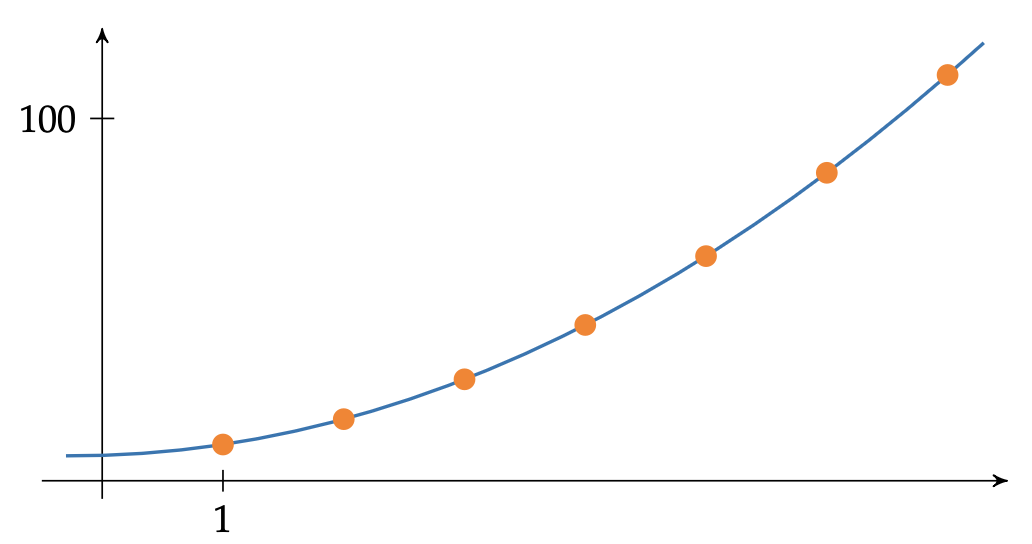
\includegraphics[width=\linewidth]{resources/images/RC_Parabel.png}
            \caption{Originale Kurve und Stützstellen}
            \label{fig:rs_original}
        \end{minipage}
        \hfill
        \begin{minipage}{0.48\textwidth}
            \centering
            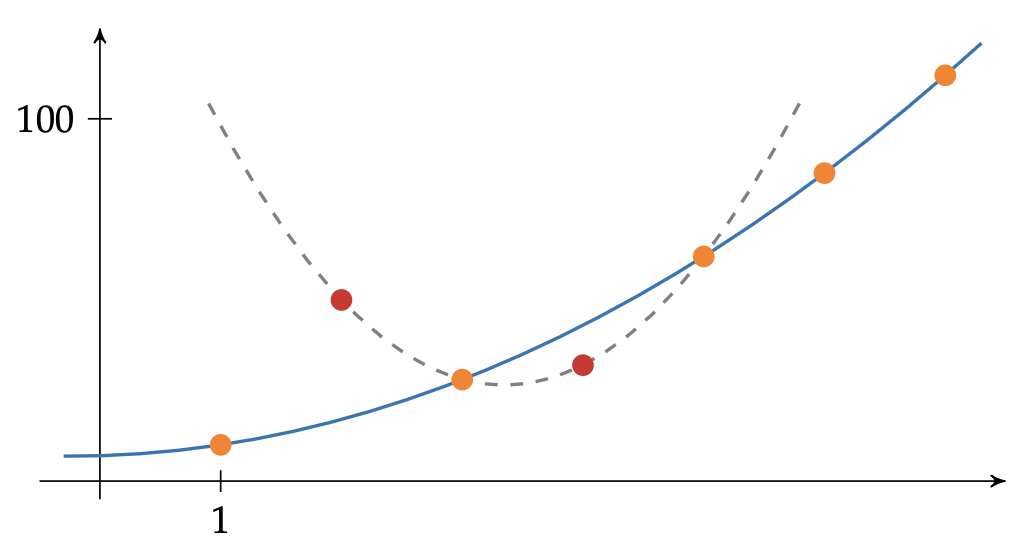
\includegraphics[width=\linewidth]{resources/images/RC_Fehlerparabel.png}
            \caption{Kurve mit fehlerhafter Stützstelle}
            \label{fig:rs_fehler}
        \end{minipage}
\end{figure}

Durch die Mehrheit der wahren Stützstellen gegenüber der fehlerhaften Stützstelle kann die ursprüngliche Kurve rekonstruiert werden. Dies ermöglicht es, die fehlerhaften Werte zu identifizieren und zu korrigieren. In diesem Beispiel können nicht mehr als zwei der richtigen Stützstellen auf der falschen Parabel liegen, dadurch ist die richtige Kurve eindeutig bestimmt. Dementsprechend ist die genaue Implementierung des Verfahrens davon abhängig, welche Arten von Fehlern erkannt und korrigiert werden sollen. Mit dem vorgestellten Beispiel ist es möglich, durch das Senden der sieben Funktionswerte \((10, 17, 28, 43, 62, 85, 112)\), die drei Zahlen \(2, 1, 7\) sicher zu übertragen. Bei unterschiedlichen Nachrichten unterscheiden sich die gesendeten Funktionswerte, aber nicht die Argumente die in der Prüfung und Berechnung verwendet werden. Die sichere Übertragung von Nachrichten aus drei Zahlen, beziehungsweise Symbolen, ist somit gewährleistet \cite{Springer_RS}.

Allgemein lässt sich dieses Verfahren wie folgt zusammenfassen: Eine Übertragung von \(k\) Symbolen, als Zahlen kodiert, nutzt eine Interpretation dieser Symbole als Polynom vom Grad \(k-1\). Der Sender sendet, um \(t\) Übertragungsfehler erfolgreich abzufangen, \(k + 2t\) Funktionswerte des Polynoms mit fest definierten Argumenten. Somit ist eine entsprechend sichere Übertragung garantiert \cite{Springer_RS}.

Um dieses Verfahren zu implementieren, muss wie beschrieben eine Polynominterpolation durchgeführt werden, um aus den Funktionswerten die ursprüngliche Nachricht zu rekonstruieren. Für eine realistische Implementierung ist eine Einschränkung nötig. Es werden in der Praxis ausschließlich endliche Körper verwendet. Dadurch ist außerdem die Anzahl der benötigten Bits für die Kodierung klar definiert. Jeder endliche Körper \(\mathbb{Z}_n\) weist mindestens eine primitive Einheitswurzel \(\alpha\) auf, für die folgendes gilt:

\begin{equation}
    \alpha^k \bmod n, \quad \text{mit } \mathbb{Z}_n \text{ und } k \in [1, n]
\end{equation}

\todo[inline]{Primitive Einheitswurzel erklären?}



